\documentclass[12pt, titlepage, french]{report}
%% -----------------------------
%% Encodage
%% -----------------------------
\usepackage[utf8]{inputenc}
\usepackage[T1]{fontenc}
\usepackage{babel}
\usepackage{lmodern}
%
%%% -----------------------------
%%% Définition de variables
%%% -----------------------------
%\def\auteur{Alec James van Rassel}
%\def\BackgroundColor{white}
%
%%% -----------------------------
%%% Margin and layout
%%% -----------------------------
%% Determine the margin for cheatsheet
%\usepackage[landscape, hmargin=1cm, vmargin=1.7cm]{geometry}
\usepackage{multicol}
\usepackage{sectsty}
\usepackage{titlesec}
%%% -----------------------------
%%%	Sections et chapitres
%%% -----------------------------
\titleformat{\chapter}
  {\normalfont\LARGE\bfseries}{\thechapter}{1em}{}
\titlespacing*{\chapter}{0pt}{3.5ex plus 1ex minus .2ex}{2.3ex plus .2ex}
\sectionfont{\color{cobalt}}
\subsectionfont{\color{indigo(web)}}
%%%
%%%	Avec cette commande, \section à le même comportement que \section* mais les sections apparaissent dans le TOC;
%%%	-	Ceci est appliqué aux sous-sections et sous-sous-sections, pas uniquement aux sections.
%
\setcounter{secnumdepth}{0}
%%%
%%%	Pour inclure les sous-sections dans la table des matières (TOC).
%%%
%%	Niveaux pour les classes book et report:
%%	-1:	part;			0:	chapter;		1:	section;			2:	subsection;	
%%	3:	subsubsection;	4:	paragraph;	5:	subparagraph;
%%	NOTE:	0 existe seulement pour les classes book et report et est part pour la class article.
%%%
\setcounter{tocdepth}{3}

%% -----------------------------
%% URL and links
%% -----------------------------
\usepackage{hyperref}
\usepackage{nameref}
\hypersetup{colorlinks = true, urlcolor = white, linkcolor = black}

%% -----------------------------
%% Document policy (en décommenter seulement une)
%% -----------------------------
%	\usepackage{concrete}
%	\usepackage{mathpazo}
%	\usepackage{frcursive} %% permet d'écrire en lettres attachées
%	\usepackage{aeguill}
%	\usepackage{mathptmx}
%	\usepackage{fourier} 

%% -----------------------------
%% Math configuration
%% -----------------------------
\usepackage[fleqn]{amsmath}
\usepackage{amsthm, amssymb, latexsym, amsfonts}
\usepackage{empheq}
\usepackage{numprint}
\usepackage{dsfont} % Pour avoir le symbole du domaine Z

%%% -----------------------------
%%% Raccourcis mathématiques
%%% -----------------------------
\newcommand{\reels}{\mathbb{R}}
\newcommand{\entiers}{\mathbb{Z}}
\newcommand{\naturels}{\mathbb{N}}
\newcommand{\eval}{\biggr \rvert}
\usepackage{cancel}
\newcommand{\derivee}[1]{\frac{\partial}{\partial #1}}
\newcommand{\prob}[1]{\Pr \left( #1 \right)}
\newcommand{\esp}[1]{\mathrm{E} \left[ #1 \right]} % espérance
\newcommand{\variance}[1]{\mathrm{Var} \left( #1   \right)}
\newcommand{\covar}[1]{\mathrm{Cov} \left( #1   \right)}
\newcommand{\laplace}{\mathcal{L}}
\newcommand{\deriv}[2][]{\frac{\partial^{#1}}{\partial #2^{#1}}}
\newcommand{\e}[1]{\mathrm{e}^{#1}}
\newcommand{\te}[1]{\text{exp}\left\{#1\right\}}
\DeclareMathSymbol{\shortminus}{\mathbin}{AMSa}{"39}

% To indicate equation number on a specific line in align environment
\newcommand\numberthis{\addtocounter{equation}{1}\tag{\theequation}}


%%% -----------------------------
%%% 	Paquetage de notation actuarielle
%%% -----------------------------
\usepackage{actuarialsymbol}
\usepackage{actuarialangle}

%%% -----------------------------
%%% Notation matricielle pour les symboles mathématiques
%%%
%%  (\bm{•})
%%% -----------------------------
\usepackage{bm}
%% Notation matricielle pour les variables
\newcommand{\matr}[1]{\mathbf{#1}}

%% -----------------------------
%% Configuration de tcolorbox
%% -----------------------------
\usepackage[most]{tcolorbox}
\tcbuselibrary{xparse}
\tcbuselibrary{breakable}
%%	-----------------------------
%%
%%	Arguments du paquetage
%%	+	breakable: allows box to be split over several pages
%%	+	segmentation style: To customize the \tcbline seperator
%%	
%%	-----------------------------
%%

%%
%% Coloured box "definition" for definitions
%%
\DeclareTColorBox{theorems}{ o}			% #1 parameter
{
	enhanced,
	title = #1,
	colback=bluebell, % color of the box
	colframe=blue(pigment),
	colbacktitle=blue!80!black,
	fonttitle = \bfseries,
	boxed title style={size=small,colframe=purple!50!black} ,
	attach boxed title to top center = {yshift=-3mm,yshifttext=-1mm},
	left=0pt,
  	right=0pt,
    box align=center,
    ams align*
%  	top=-10pt
}
\DeclareTColorBox{distributions}{ o }			% #1 parameter
{
	enhanced,
	title = #1,
	colback=ashgrey, % color of the box
%	colframe=blue(pigment),
	breakable,
	colframe=arsenic,	
	colbacktitle=aurometalsaurus,
	fonttitle = \bfseries,
	boxed title style={size=small,colframe=arsenic} ,
	attach boxed title to top center = {yshift=-3mm,yshifttext=-1mm},
%	left=0pt,
%  	right=0pt,
%    box align=center,
%    ams align*
%  	top=-10pt
}
\DeclareTColorBox{outcomes}{ o }			% #1 parameter
{
	enhanced,
	title = #1,
	colback=bluebell, % color of the box
%	colframe=blue(pigment),
%	colframe=asparagus,	
	breakable,
	colbacktitle=airforceblue,
	fonttitle = \bfseries,
	boxed title style={size=small,colframe=arsenic} ,
	attach boxed title to top center = {yshift=-3mm,yshifttext=-1mm},
%	left=0pt,
%  	right=0pt,
%    box align=center,
%    ams align*
%  	top=-10pt
}
\DeclareTColorBox{ASM_chapter}{ o }			% #1 parameter
{
	enhanced,
	title = #1,
	colback=darkseagreen, % color of the box
%	colframe=blue(pigment),
%	colframe=asparagus,	
	colbacktitle=britishracinggreen,
	fonttitle = \bfseries,
	boxed title style={size=small,colframe=arsenic} ,
	attach boxed title to top center = {yshift=-3mm,yshifttext=-1mm},
	segmentation style = {dashed, white},
	breakable
%	left=0pt,
%  	right=0pt,
%    box align=center,
%    ams align*
%  	top=-10pt
}
\DeclareTColorBox{YTB_vids}{ o }			% #1 parameter
{
	enhanced,
	title = #1,
	colback=red_rectangle, % color of the box
%	colframe=blue(pigment),
%	colframe=asparagus,	
	colbacktitle=lava,
	fonttitle = \bfseries,
	boxed title style={size=small,colframe=arsenic} ,
	attach boxed title to top center = {yshift=-3mm,yshifttext=-1mm},
	segmentation style = {dashed, white},
	breakable
%	left=0pt,
%  	right=0pt,
%    box align=center,
%    ams align*
%  	top=-10pt
}
%%
%% Coloured box "algo" for algorithms
%%
\newtcolorbox{algo}[ 1 ]
{
	colback = blue!5!white,
	colframe = blue!75!black,
	fonttitle = \bfseries,title=#1
}
%%
%% Coloured box "formula" for formulas
%%
\newtcolorbox{formula}[ 1 ]
{
	colback = green!5!white,
	colframe = darkseagreen,
	fonttitle = \bfseries,title=#1
}
%%
%% Coloured box "CHPT_SUMM" pour résumés des chapitres de l'ASM
%%
%\newtcolorbox[auto counter]{CHPT_SUMM}[ 2 ][] 	%pour ajouter du numérotage automatique
\newtcolorbox{CHPT_SUMM}[ 2 ][]
{
	colback = green!5!white,
	colframe = darkseagreen,
	breakable,
	enhanced,
	fonttitle = \bfseries,
%	title = Chapitre~\thetcbcounter: #2, 		pour inclure le numérotage automatique
	title = #2,
	#1
}
\newtcolorbox[list inside = CHPT]{CHPT_SUMM_AUTO}[ 2 ][]
{
	colback = green!5!white,
	colframe = darkseagreen,
	breakable,
	enhanced,
	fonttitle = \bfseries,
%	title = Chapitre~\thetcbcounter: #2, 		pour inclure le numérotage automatique
	title = #2,
	nameref = #2,
	after upper = {\addcontentsline{toc}{subsubsection}{#2}},
%	phantomlabel = {#2},
	#1
}
\newtcolorbox[auto counter, list inside = CHPT]{CHPT_SUMM_AUTO_NUMB}[ 2 ][]
{
	colback = green!5!white,
	colframe = darkseagreen,
	breakable,
	enhanced,
	fonttitle = \bfseries,
	title = Chapter~\thetcbcounter: #2, 		
%	title = #2,
	nameref = #2,
	after upper = {\addcontentsline{toc}{subsubsection}{\thetcbcounter: #2}},
%	phantomlabel = {#2},
	#1
}
%%
%% Coloured box "FORMULA_SUMM" pour résumés des formules de l'ASM
%%
\newtcolorbox{FORMULA_SUMM}[ 1 ]
{
	colback = babyblueeyes,
	colframe = airforceblue,
	breakable,
	fonttitle = \bfseries,title=#1
}
%%
%% Coloured box "YTB_SUMM" pour résumés des vidéos Youtube
%%
\newtcolorbox{YTB_SUMM}[ 2 ][]
{
	colback = red!5!white,
	colframe = darkterracotta,
	breakable,
	enhanced,
%	    frame hidden,
	fonttitle = \bfseries,
	title=#2,
	#1
}

%% -----------------------------
%% Graphiques et images
%% -----------------------------
\usepackage{graphicx}
\usepackage{pict2e}
\usepackage{tikz}

%%
%%	Crée un cercle
%%	Arguments:
%%	+	size
%%	+	colour
%%	
%%	Example:
%%	+	\tikzcircle[green, fill=blue]{1.5pt}
%%	+	\tikzcircle{2pt}
%%
\newcommand{\tikzcircle}[2][red,fill=red]{\tikz[baseline=-0.5ex]\draw[#1,radius=#2] (0,0) circle ;}

%%% -----------------------------
%%% insérer des pages pdf dans un document
%%% -----------------------------
\usepackage{pdfpages}

%%% -----------------------------
%%% Color configuration
%%% -----------------------------
\usepackage{color, soulutf8, colortbl}

%%% -----------------------------
%%%	Définitions de couleurs
%%% -----------------------------
\definecolor{darkterracotta}{rgb}{0.8, 0.31, 0.36}   % red pastel ish
\definecolor{lava}{rgb}{0.81, 0.06, 0.13}
\definecolor{wildwatermelon}{rgb}{0.99, 0.42, 0.52}  % red ish
\definecolor{bostonuniversityred}{rgb}{0.8, 0.0, 0.0} % rich red
\definecolor{asparagus}{rgb}{0.53, 0.66, 0.42}		% sorta militarygreen but pastel
\definecolor{darkseagreen}{rgb}{0.56, 0.74, 0.56}    % pastel light green
\definecolor{britishracinggreen}{rgb}{0.0, 0.26, 0.15} %dark green
\definecolor{airforceblue}{rgb}{0.36, 0.54, 0.66}	% nice teal blue pastel
\definecolor{babyblueeyes}{rgb}{0.63, 0.79, 0.95}	% pastel blue-ish
\definecolor{applegreen}{rgb}{0.55, 0.71, 0.0}		% green with some aqua
\definecolor{indigo(web)}{rgb}{0.29, 0.0, 0.51}
\definecolor{cobalt}{rgb}{0.0, 0.28, 0.67}
\definecolor{azure(colorwheel)}{rgb}{0.0, 0.5, 1.0}
\definecolor{darkpastelpurple}{rgb}{0.59, 0.44, 0.84}
\definecolor{darkgreen}{rgb}{0.0, 0.2, 0.13}			
\definecolor{burntorange}{rgb}{0.8, 0.33, 0.0}		
\definecolor{burntsienna}{rgb}{0.91, 0.45, 0.32}		
\definecolor{ao(english)}{rgb}{0.0, 0.5, 0.0}		% ACT-2003
\definecolor{amber(sae/ece)}{rgb}{1.0, 0.49, 0.0} 	% ACT-2004
\definecolor{green_rectangle}{RGB}{131, 176, 84}		% ACT-2004
\definecolor{red_rectangle}{RGB}{241,112,113}		% ACT-2004
\definecolor{blue_rectangle}{RGB}{83, 84, 244}		% ACT-2004
\definecolor{blue(pigment)}{rgb}{0.2, 0.2, 0.6}
\definecolor{bluebell}{rgb}{0.64, 0.64, 0.82}
\definecolor{amethyst}{rgb}{0.6, 0.4, 0.8}
\definecolor{amethyst-light}{rgb}{0.6, 0.4, 0.8}
\definecolor{aurometalsaurus}{rgb}{0.43, 0.5, 0.5}
\definecolor{arsenic}{rgb}{0.23, 0.27, 0.29}			%	dark black-grey ish pastel
\definecolor{ashgrey}{rgb}{0.7, 0.75, 0.71}
%
% Useful shortcuts for coloured text
%
\newcommand{\orange}{\textcolor{orange}}
\newcommand{\red}{\textcolor{red}}
\newcommand{\cyan}{\textcolor{cyan}}
\newcommand{\blue}{\textcolor{blue}}
\newcommand{\green}{\textcolor{green}}
\newcommand{\purple}{\textcolor{magenta}}
\newcommand{\yellow}{\textcolor{yellow}}

%% -----------------------------
%% Enumerate environment configuration
%% -----------------------------
%
% Custum enumerate & itemize Package
%
\usepackage{enumitem}
%
% French Setup for itemize function
%
\frenchbsetup{StandardItemLabels=true}
%
% Change default label for itemize
%
\renewcommand{\labelitemi}{\faAngleRight}


%% -----------------------------
%% Tabular column type configuration
%% -----------------------------
\newcolumntype{C}{>{$}c<{$}} % math-mode version of "l" column type
\newcolumntype{L}{>{$}l<{$}} % math-mode version of "l" column type
\newcolumntype{R}{>{$}r<{$}} % math-mode version of "l" column type
\newcolumntype{f}{>{\columncolor{green!20!white}}p{1cm}}
\newcolumntype{g}{>{\columncolor{green!40!white}}m{1.2cm}}
\newcolumntype{a}{>{\columncolor{red!20!white}$}p{2cm}<{$}}	% ACT-2005
% configuration to force a line break within a single cell
\usepackage{makecell}


%% -----------------------------
%% Fontawesome for special symbols
%% -----------------------------
\usepackage{fontawesome}

%
%%% -----------------------------
%%% Footer/Header Customization
%%% -----------------------------
%\usepackage{lastpage}
%\usepackage{fancyhdr}
%\pagestyle{fancy}
%%
%% Page background color
%%
%\pagecolor{\BackgroundColor}


%% END OF PREAMBLE
% ---------------------------------------------
% ---------------------------------------------
%% -----------------------------
%% Section Font customization
%% -----------------------------
\title{
	Guide d'étude	\\
	\large Examen MAS-I: Modern Actuarial Statistics I\\
	Casualty Actuarial Society (CAS)}
\vspace{-8ex}
\date{}
\author{Alec James van Rassel}

\begin{document}

\maketitle

\tableofcontents

\clearpage

\part*{Préliminaire}

\section{Information}

\begin{distributions}[Objectives]
\begin{itemize}
	\item	Set forth, usually in broad terms, what the candidate should be able to do in actual practice;
	\item	The objectives include methodologies that may be impossible to perform on an exam that the candidate is expected to be able to explain conceptually;
	\item	\textit{For example}: The Hat Matrix couldn't be calculated, but conceptual questions about it could be asked;
\end{itemize}
\end{distributions}

\begin{outcomes}[Learning outcomes]
\begin{enumerate}
	\item	It's important to identify some of the key terms, concepts, and methods associated with each of the learning objectives;
	\item	They aren't an exhaustive list of the material being tested, but rather illustrate the scope of each learning objective;
\end{enumerate}
\end{outcomes}

\begin{CHPT_SUMM}{Information additionnelle}
	\begin{itemize}
		\item	The learning objectives define the behaviours and the knowledge statements illustrate more fully their intended scope;
		\item	Learning objectives should not be seen as independent units but as building blocks for our understanding;
		\item	The ranges are just guidelines;
		\item	The overall section weights should be seen as having more significance than the individual section weights;
		\item	Tables include :
			\begin{itemize}
			\item	values for the illustrative life tables;
			\item	Standard normal distribution;
			\item	Abridged inventories of discrete and continuous probability distributions;
			\item	Chi-square distribution;
			\item	$t$-distribution;
			\item	$F$-distribution;
			\end{itemize}
		\item	\textbf{There is a guessing adjustment};
	\end{itemize}
\end{CHPT_SUMM}

\part*{Sujets à l'étude}

\chapter[Probability models (Stochastic Processes and Survival Models)]{Probability models (Stochastic Processes and Survival Models) (20\% à 35\%)}

\subsection{Information}

\begin{distributions}[Description]
Notes du descriptif principal:
\begin{itemize}
	\item	Stochastic processes
	\item	Survival models
		\begin{itemize}
		\item	Covered in depth as part of probability modeling in generic terms;
		\end{itemize}
	\item	Markov Chains
		\begin{itemize}
		\item	Provide the means to model how an entity can move through different states;
		\end{itemize}
	\item	Simplified version of life contingencies
		\begin{itemize}
		\item	Life contingencies problems can be viewed as discounted cash flow problems which include thee effect of probability of payment;
		\item	Covered through a study note which link the generic survival model concepts to a subset of life actuarial concepts;
		\item	This study note illustrates how to calculate annuities or single premium insurance amounts;
		\end{itemize}
\end{itemize}
\tcbline
Notes de la sous-section:
\begin{itemize}
	\item	Résoudre des problèmes de processus aléatoires;
	\item	Identifier les probabilités et distributions associées avec ces processus;
		\begin{itemize}
		\item	Particulièrement, être capable d'utiliser un processus de Poisson dans ces applications;
		\end{itemize}
	\item	Les modèles de survie sont une rallonge aux modèles de probabilité de processus stochastiques;
		\begin{itemize}
		\item	En lieu, on estime la vie futur d'une entité avec quelques suppositions sur la distribution de la vraisemblance de survie;
		\end{itemize}
	\item	Chaines de Markov utiles pour modéliser la mobilité entre états dans un processus et souligner les modèles Bayésien MCMC sous-jacent;
	\item	La simulation est incluse puisqu'elle peut s'avérer essentielle pour arriver à une solution de problème complexe;
\end{itemize}
\end{distributions}


\begin{outcomes}[Learning objectives]
\begin{enumerate}
	\item	Understand and apply the properties of Poisson processes;
		\begin{itemize}
		\item	For increments in the homogeneous case;
		\item	For interval times in the homogeneous case;
		\item	For increments in the non-homogeneous case;
		\item	Resulting from special types of events in the Poisson process;
		\item	Resulting from sums of independent Poisson processes;
		\end{itemize}
	\begin{knowledge}[Knowledge Statements]
	\begin{enumerate}[label = \alph*.]
		\item	Poisson process;
		\item	Non-homogeneous Poisson process;
		\item	Memoryless property of Exponential and Poisson;
		\item	Relationship between Exponential and Gamma;
		\item	Relationship between Exponential and Poisson;
	\end{enumerate}
	\end{knowledge}
\tcbline
	\item	For any Poisson process and the inter-arrival and waiting distributions associated with the Poisson process, calculate:
		\begin{itemize}
		\item	Expected values;
		\item	Variances;
		\item	Probabilities;
		\end{itemize}
	\begin{knowledge}[Knowledge Statements]
	\begin{enumerate}[label = \alph*.]
		\item	Probability calculations for Poisson process
		\item	Conditional distribution of arrival times;
		\item	Splitting grouped Poisson rate to subsets of population using probability distribution;
		\item	Conditional distribution of events by category within a group within a certain time period;
	\end{enumerate}
	\end{knowledge}
\tcbline
	\item	For a compound Poisson process, calculate moments associated with the value of the process at a given time;
	\begin{knowledge}[Knowledge Statements]
	\begin{enumerate}[label = \alph*.]
		\item	Compound Poisson process mean and variance;
		\item	Normal approximation and hypothesis testing;
	\end{enumerate}
	\end{knowledge}
\tcbline
	\item	Apply the Poisson process concepts to calculate the hazard function and related survival model concepts;
		\begin{itemize}
		\item	Relationship between hazard rate, probability density function and cumulative distribution function;
		\item	Effect of memoryless nature of Poisson distribution on survival time estimation;
		\end{itemize}
	\begin{knowledge}[Knowledge Statements]
	\begin{enumerate}[label = \alph*.]
		\item	Failure time random variables;
		\item	Cumulative distribution functions;
		\item	Survival functions;
		\item	Probability density functions;
		\item	Hazard functions and relationship to Exponential distribution;
		\item	Relationships between failure time random variables in the functions above;
		\item	Greedy algorithms;
	\end{enumerate}
	\end{knowledge}
\tcbline
	\item	Given the joint distribution of more than one source of failure in a system (or life) and using Poisson Process assumptions:
		\begin{itemize}
		\item	Calculate probabilities and moments associated with functions of these random variables' variances;
		\item	Understand differences between a series system (joint life) and parallel system (last survivor) when calculating expected time to failure or probability of failure by a certain time;
		\item	Understand the effect of multiple sources of failure (multiple decrement) on expected system time to failure (expected lifetime);
		\end{itemize}
	\begin{knowledge}[Knowledge Statements]
	\begin{enumerate}[label = \alph*.]
		\item	Joint distribution of failure times;
		\item	Probabilities and moments;
		\item	Time until failure of the system (life);
		\item	Time until failure of the system (life) from a specific cause;
		\item	Time until failure of the system (life) for parallel or series systems with multiple components;
		\item	Paths that lead to parallel or series system failures for systems with multiple components;
		\item	Relationship between failure time and minimal path and minimal cut sets;
		\item	Bridge system and defining path to failure;
		\item	Random graphs and defining path to failure;
		\item	Effect of multiple sources of failure (multiple decrements) on failure time calculations (competing risk);
		\item	Non-uniform probability of component failure (multiple decrement);
		\item	Method of inclusion and exclusion as applied to failure time estimates;
		\item	Expected system lifetime as function of component lifetime and properties of expected lifetime estimates;
		\item	Linkage between reliability function for a system and future expected lifetime;
	\end{enumerate}
	\end{knowledge}
\tcbline
	\item	For discrete Markov Chains under both homogeneous and non-homogenous states:	
		\begin{itemize}
		\item	Definition of a Markov Chain;
		\item	Chapman-Kolmogorov Equations for $n$-step transition calculations;
		\item	Accessible states;
		\item	Ergodic Markov Chains and limiting probabilities;
		\end{itemize}
	\begin{knowledge}[Knowledge Statements]
	\begin{enumerate}[label = \alph*.]
		\item	Random Walk;
		\item	Classification of states and classes of states (absorbing, accessible, transition, irreducible, and recurrent);
		\item	Transition step probabilities;
		\item	Stationary probabilities;
		\item	Recurrent vs. transient states;
		\item	Gamblers ruin problem;
		\item	Branching processes;
		\item	Homogeneous transition probabilities;
		\item	Memoryless property of Markov Chains;
		\item	Limiting probabilities;
	\end{enumerate}
	\end{knowledge}
\tcbline
	\item	Solve Life Contingency problems using a life table in a spreadsheet as the combined result of discount, probability of payment and amount of payment vectors. Understand the linkage between the life table and the corresponding probability models;
		\begin{itemize}
		\item	Calculate annuities for discrete time;
		\item	Calculate life insurance single net premiums (or P \& C pure premiums) for discrete time;
		\item	Solve for net level premiums (\textbf{not} including fractional lives);
		\end{itemize}
	\begin{knowledge}[Knowledge Statements]
	\begin{enumerate}[label = \alph*.]
		\item	Discounted cash flow;
		\item	Relationship between annuity values and insurance premiums;
		\item	Life table linkage to probability models;
		\item	Equivalence property;
	\end{enumerate}
	\end{knowledge}
\tcbline
	\item	The candidate should be familiar with basic computer simulation methods.
		\begin{itemize}
		\item	Understand the basic framework of Monte Carlo Simulation;
		\item	Understand the mechanics of generating uniform random numbers;
		\item	Generate random numbers from a variety of distributions using the inversion method;
		\item	Be able to explain when and how to use the Acceptance-Rejection method;
		\end{itemize}
	\begin{knowledge}[Knowledge Statements]
	\begin{enumerate}[label = \alph*.]
		\item	Random Number Generation;
		\item	Uniform Random Numbers;
		\item	Inversion Method;
		\item	Acceptance-Rejection Method;
	\end{enumerate}
	\end{knowledge}
\end{enumerate}
\end{outcomes}

\begin{ASM_chapter}[Related lessons ASM]
\begin{enumerate}
	\item	\nameref{L.-1}
	\item	\nameref{L.-2}
	\item	\nameref{L.-3}
\tcbline
	\item	\nameref{L.-4}
	\item	\nameref{L.-5}
	\item	\nameref{L.-6}
	\item	\nameref{L.-7}
	\item	\nameref{L.-8}
	\item	\nameref{L.-9}
	\item	\nameref{L.-10}
	\item	\nameref{L.-11}
	\item	\nameref{L.-12}
	\item	\nameref{L.-13}
	\item	\nameref{L.-14}
	\item	\nameref{L.-15}
	\item	\nameref{L.-16}
	\item	\nameref{L.-17}
	\item	\nameref{L.-18}
	\item	\nameref{L.-19}
\tcbline
	\item	\nameref{L.-20}
	\item	\nameref{L.-21}
\tcbline
	\item	\nameref{L.-22}
	\item	\nameref{L.-23}
	\item	\nameref{L.-24}
\end{enumerate}
\end{ASM_chapter}

\begin{YTB_vids}[Vidéos YouTube]
\begin{itemize}
	\item	
\end{itemize}
\end{YTB_vids}

\subsection{Résumés des chapitres}

\subsubsection*{Probability Review}

\begin{CHPT_SUMM_AUTO_NUMB}[label = {L.-1}]{Probability Review}
Introduction to Mathematical Statistics 1 - 3, 5
	\begin{itemize}
		\item	
	\end{itemize}
\end{CHPT_SUMM_AUTO_NUMB}

\begin{CHPT_SUMM_AUTO_NUMB}[label = {L.-2}]{Parametric Distributions}
Introduction to Mathematical Statistics 2.2, 2.7
Nonlife Actuarial Models---Theory Methods and Evaluation 2.2
	\begin{itemize}
		\item	
	\end{itemize}
\end{CHPT_SUMM_AUTO_NUMB}

\begin{CHPT_SUMM_AUTO_NUMB}[label = {L.-3}]{Mixtures}
Introduction to Mathematical Statistics 3.7
Nonlife Actuarial Models---Theory Methods and Evaluation 2.3.2
	\begin{itemize}
		\item	
	\end{itemize}
\end{CHPT_SUMM_AUTO_NUMB}

\subsubsection*{Stochastic Processes}

\begin{CHPT_SUMM_AUTO_NUMB}[label = {L.-4}]{Markov Chains: Chapman-Kolmogorov Equations}
Ross 4.1 - 4.2, 4.5.1 - 4.5.2
	\begin{itemize}
		\item	
	\end{itemize}
\end{CHPT_SUMM_AUTO_NUMB}

\begin{CHPT_SUMM_AUTO_NUMB}[label = {L.-5}]{Markov Chains: Classification of States}
Ross 4.3
	\begin{itemize}
		\item	
	\end{itemize}
\end{CHPT_SUMM_AUTO_NUMB}

\begin{CHPT_SUMM_AUTO_NUMB}[label = {L.-6}]{Discrete Markov Chains: Long-Run Proportions and Limiting Probabilities}
Ross 4.4
	\begin{itemize}
		\item	
	\end{itemize}
\end{CHPT_SUMM_AUTO_NUMB}

\begin{CHPT_SUMM_AUTO_NUMB}[label = {L.-7}]{Markov Chains: Time in Transient States}
Ross 4.6
	\begin{itemize}
		\item	
	\end{itemize}
\end{CHPT_SUMM_AUTO_NUMB}

\begin{CHPT_SUMM_AUTO_NUMB}[label = {L.-8}]{Markov Chains: Branching Processes}
Ross 4.7
	\begin{itemize}
		\item	
	\end{itemize}
\end{CHPT_SUMM_AUTO_NUMB}

\begin{CHPT_SUMM_AUTO_NUMB}[label = {L.-9}]{Markov Chains: Time Reversible}
Ross 4.8
	\begin{itemize}
		\item	
	\end{itemize}
\end{CHPT_SUMM_AUTO_NUMB}

\begin{CHPT_SUMM_AUTO_NUMB}[label = {L.-10}]{Exponential Distribution}
Ross 5.2
	\begin{itemize}
		\item	
	\end{itemize}
\end{CHPT_SUMM_AUTO_NUMB}

\begin{CHPT_SUMM_AUTO_NUMB}[label = {L.-11}]{The Poisson Process: Probabilities of Events}
Ross 5.3.1 - 5.3.2
Daniel Poisson Study Note 1.1, 1.4.1
	\begin{itemize}
		\item	
	\end{itemize}
\end{CHPT_SUMM_AUTO_NUMB}

\begin{CHPT_SUMM_AUTO_NUMB}[label = {L.-12}]{The Poisson Process: Time To Next Event}
Ross 5.2, 5.3.3
Daniel Poisson Study Note 1.1.1
	\begin{itemize}
		\item	
	\end{itemize}
\end{CHPT_SUMM_AUTO_NUMB}

\begin{CHPT_SUMM_AUTO_NUMB}[label = {L.-13}]{{The Poisson Process: Thinning, or Couting Special Types of Events}}
Ross 5.3.4
Daniel Poisson Study Note 1.3.1, 1.4.3
	\begin{itemize}
		\item	
	\end{itemize}
\end{CHPT_SUMM_AUTO_NUMB}

\begin{CHPT_SUMM_AUTO_NUMB}[label = {L.-14}]{The Poisson Process: Other Characteristics}
Ross 5.2.3, 5.3.4, 5.3.5
	\begin{itemize}
		\item	
	\end{itemize}
\end{CHPT_SUMM_AUTO_NUMB}

\begin{CHPT_SUMM_AUTO_NUMB}[label = {L.-15}]{The Poisson Process: Sums and Mixtures}
Ross 5.4.3
Daniel Poisson Study Note 1.3.2, 1.3.3
	\begin{itemize}
		\item	
	\end{itemize}
\end{CHPT_SUMM_AUTO_NUMB}

\begin{CHPT_SUMM_AUTO_NUMB}[label = {L.-16}]{Compound Poisson Processes}
Ross 5.4.2
Daniel Poisson Study Note 1.2, 1.4.2
	\begin{itemize}
		\item	
	\end{itemize}
\end{CHPT_SUMM_AUTO_NUMB}

\begin{CHPT_SUMM_AUTO_NUMB}[label = {L.-17}]{Reliability: Structure Functions}
Ross 9.1 - 9.2
	\begin{itemize}
		\item	
	\end{itemize}
\end{CHPT_SUMM_AUTO_NUMB}

\begin{CHPT_SUMM_AUTO_NUMB}[label = {L.-18}]{Reliability: Probabilities}
Ross 9.3 - 9.4
	\begin{itemize}
		\item	
	\end{itemize}
\end{CHPT_SUMM_AUTO_NUMB}

\begin{CHPT_SUMM_AUTO_NUMB}[label = {L.-19}]{Reliability: Time to Failure}
Ross 9.5 - 9.6
	\begin{itemize}
		\item	
	\end{itemize}
\end{CHPT_SUMM_AUTO_NUMB}

\subsubsection*{Life Contingencies}

\begin{CHPT_SUMM_AUTO_NUMB}[label = {L.-20}]{Survival Models}
Struppeck 1, 2, 6, 7
	\begin{itemize}
		\item	
	\end{itemize}
\end{CHPT_SUMM_AUTO_NUMB}

\begin{CHPT_SUMM_AUTO_NUMB}[label = {L.-21}]{Contingent Payments}
Struppeck 3, 4, 5, 6
	\begin{itemize}
		\item	
	\end{itemize}
\end{CHPT_SUMM_AUTO_NUMB}

\subsubsection*{Simulation}

\begin{CHPT_SUMM_AUTO_NUMB}[label = {L.-22}]{Simulation---Inverse Transformation Method}
Ross 11.1, 11.2.1
	\begin{itemize}
		\item	
	\end{itemize}
\end{CHPT_SUMM_AUTO_NUMB}

\begin{CHPT_SUMM_AUTO_NUMB}[label = {L.-23}]{Simulation---Applications}
Ross 11.1, 11.2.1
	\begin{itemize}
		\item	
	\end{itemize}
\end{CHPT_SUMM_AUTO_NUMB}

\begin{CHPT_SUMM_AUTO_NUMB}[label = {L.-24}]{Simulation---Rejection Method}
Ross 11.2.2
	\begin{itemize}
		\item	
	\end{itemize}
\end{CHPT_SUMM_AUTO_NUMB}

\subsection{Notes sur les vidéos YouTube}

\begin{YTB_SUMM}[label = {SQ-BASICS-ML-INTRO}]{\href{https://www.youtube.com/watch?v=Gv9_4yMHFhI&list=PLblh5JKOoLUICTaGLRoHQDuF_7q2GfuJF&index=2&t=0s}{StatQuest: A Gentle Introduction to Machine Learning}}
\begin{itemize}
	\item	
\end{itemize}
\end{YTB_SUMM}

\newpage

\chapter[Statistics]{Statistics (15\% à 30\%)}

\subsection{Information}

\begin{distributions}[Description]
Notes du descriptif principal:
\begin{itemize}
	\item	Topics which would commonly be covered in a 2-semester Probability \& Statistics sequence;
\end{itemize}
\end{distributions}

\begin{outcomes}[Learning objectives]
\begin{enumerate}
	\item	Perform point estimation of statistical parameters using Maximum likelihood estimation (MLE). Apply criteria to estimates such as :
	\begin{multicols*}{2}
		\begin{itemize}
		\item	Consistency;
		\item	Unbiasedness;
		\item	Sufficiency;
		\item	Efficiency;
		\item	Minimum variance;
		\item	MSE;
		\end{itemize}
	\end{multicols*}
	\begin{knowledge}[Knowledge Statements]
	\begin{enumerate}[label = \alph*.]
	\item	Equations for MLE of mean, variance from a sample;
	\item	Estimation of mean and variance based on samples;
	\item	General equations for MLE of parameters;
	\item	Recognition of consistency property of estimators and alternative measures of consistency;
	\item	Application of criteria for measurement when estimating parameters through minimisation of variance, MSE;
	\item	Definition of statistical bias and recognition of estimators that are unbiased or biased;
	\item	Application of Rao-Cramer Lower Bound and Efficiency;
	\item	Relationship between Sufficiency and Minimum Variance;
	\item	Develop and estimate a sufficient statistic for a distribution;
	\item	Factorization Criterion for sufficiency;
	\item	Application of Rao-Cramer Lower Bound and Fisher Information;
	\item	Application of MVUE for the exponential class of distributions;
	\item	Linkage between Score Function, Fisher Information and maximum likelihood;
	\item	Method of Moments;
	\item	Percentile Matching;
	\item	Kernel Density Estimation;
	\item	Maximum Likelihood with Censoring and Truncation;
	\end{enumerate}
	\end{knowledge}
\tcbline
	Calculate parameter estimates using methods other than maximum likelihood;
	\item	Test statistical hypotheses including Type I and Type II errors using:
		\begin{itemize}
		\item	Neyman-Pearson theorem;
		\item[]	Apply Neyman-Pearson theorem to construct likelihood ratio equation;
		\item	Likelihood ratio tests;
		\item	First principles;
		\item[]	Use critical values from a sampling distribution to test means and variances;
		\end{itemize}		
	\begin{knowledge}[Knowledge Statements]
	\begin{enumerate}[label = \alph*.]
	\item	Presentation of fundamental inequalities based on general assumptions and normal assumptions;
	\item	Definition of Type I and Type II errors;
	\item	Significance levels;
	\item	One-sided versus two-sided tests;
	\item	Estimation of sample sizes under normality to control for Type I and Type II errors;
	\item	Determination of critical regions;
	\item	Definition and measurement of likelihood ratio tests;
	\item	Determining parameters and testing using tabular values (from a table);
	\item	Recognizing when to apply likelihood ratio tests versus chi-square or other goodness of fit tests;
	\item	Apply paired $t$-test to two samples;
	\item	Test for difference in variance under Normal distribution between two samples through the application of $F$-test;
	\item	Test of significance of means from two samples under Normal distribution assumptions in both large and small sample cases;
	\item	Test for significance of difference in proportions between two samples under the Binomial distribution assumption in both large and small sample cases;
	\item	Application of contingency tables to test independence between effects;
	\item	Asymptotic relationship between likelihood ratio tests and the Chi-Square distribution;
	\item	Application of Neyman-Pearson theorem to Uniformly Most Powerful hypothesis tests;
	\item	Equivalence between critical regions and confidence intervals;
	\item	Kolmogorov-Smirnov test;
	\end{enumerate}
	\end{knowledge}
\tcbline
	\item	For the Exponential, Gamma, Weibull, Pareto, Lognormal, Beta, and mixtures thereof:
		\begin{itemize}
		\item	Identify the applciations to Insurance claim modeling in which each distribution is used and reasons why;
		\item	Transformation of distributions; 
		\end{itemize}
	\begin{knowledge}[Knowledge Statements]
	\begin{enumerate}[label = \alph*.]
	\item	Frequency, severity and aggregate loss;
	\item	Common continuous distributions for modeling claim severity;
	\item	Mixing distributions;
	\item	Tail properties of claim severity;
	\item	Effects of coverage modifications including, for example: limits, deductibles, loss elimination ratios and effects of inflation;
	\end{enumerate}
	\end{knowledge}
\tcbline
	\item	Calculate Order Statistics of a sample for a given distribution;
	\begin{knowledge}[Knowledge Statements]
	\begin{enumerate}[label = \alph*.]
	\item	General form for distribution of $n^{\text{th}}$ largest element of a set;
	\item	Application to a given distributional form;
	\end{enumerate}
	\end{knowledge}
\end{enumerate}
\end{outcomes}

\begin{ASM_chapter}[Related lessons ASM]
\begin{enumerate}
  \setcounter{enumi}{24}
	\item	\nameref{L.-25}
	\item	\nameref{L.-26}
	\item	\nameref{L.-27}
	\item	\nameref{L.-28}
	\item	\nameref{L.-29}
	\item	\nameref{L.-30}
	\item	\nameref{L.-31}
	\item	\nameref{L.-32}
	\item	\nameref{L.-33}
	\item	\nameref{L.-34}
	\item	\nameref{L.-35}
	\item	\nameref{L.-36}
	\item	\nameref{L.-37}
	\item	\nameref{L.-38}
	\item	\nameref{L.-39}
	\item	\nameref{L.-40}
	\item	\nameref{L.-41}
\end{enumerate}
\end{ASM_chapter}

\begin{YTB_vids}[Vidéos YouTube]
\begin{itemize}
	\item	
\end{itemize}
\end{YTB_vids}

\begin{distributions}[Likely Questions]
\begin{itemize}
	\item	Question where we calculate the sample variance with the STAT function of the calculator;
		\begin{itemize}
		\item	MAS-I F19, \# 15	;
		\end{itemize}
\end{itemize}
\end{distributions}

\subsection{Résumés des chapitres}

\begin{CHPT_SUMM_AUTO_NUMB}[label = {L.-25}]{Estimator Quality}
Introduction to Mathematical  4.1.3, 5.1, 7.1
	\begin{itemize}
		\item	
	\end{itemize}
\end{CHPT_SUMM_AUTO_NUMB}

\begin{CHPT_SUMM_AUTO_NUMB}[label = {L.-26}]{Kernel Density Estimation}
Nonlife Actuarial Models: Theory Methods and Evaluation 11.1
	\begin{itemize}
		\item	
	\end{itemize}
\end{CHPT_SUMM_AUTO_NUMB}

\begin{CHPT_SUMM_AUTO_NUMB}[label = {L.-27}]{Method of Moments}
Nonlife Actuarial Models: Theory Methods and Evaluation 12.1.1
	\begin{itemize}
		\item	
	\end{itemize}
\end{CHPT_SUMM_AUTO_NUMB}

\begin{CHPT_SUMM_AUTO_NUMB}[label = {L.-28}]{Percentile Matching}
Nonlife Actuarial Models: Theory Methods and Evaluation 11.1.1, 12.1.2
	\begin{itemize}
		\item	
	\end{itemize}
\end{CHPT_SUMM_AUTO_NUMB}

\begin{CHPT_SUMM_AUTO_NUMB}[label = {L.-29}]{Maximum Likelihood Estimators}
Introduction to Mathematical Statistics 4.1, 6.1
Nonlife Actuarial Models: Theory Methods and Evaluation 10.2, 12.3
	\begin{itemize}
		\item	
	\end{itemize}
\end{CHPT_SUMM_AUTO_NUMB}

\begin{CHPT_SUMM_AUTO_NUMB}[label = {L.-30}]{Maximum Likelihood Estimators---Special Techniques}
Introduction to Mathematical Statistics 4.1, 6.1
Nonlife Actuarial Models: Theory Methods and Evaluation 10.2, 12.3
	\begin{itemize}
		\item	
	\end{itemize}
\end{CHPT_SUMM_AUTO_NUMB}

\begin{CHPT_SUMM_AUTO_NUMB}[label = {L.-31}]{Variance of Maximum Likelihood Estimator}
Introduction to Mathematical Statistics 6.2, 6.5
	\begin{itemize}
		\item	
	\end{itemize}
\end{CHPT_SUMM_AUTO_NUMB}

\begin{CHPT_SUMM_AUTO_NUMB}[label = {L.-32}]{Sufficient Statistics}
Introduction to Mathematical Statistics 7
	\begin{itemize}
		\item	
	\end{itemize}
\end{CHPT_SUMM_AUTO_NUMB}

\begin{CHPT_SUMM_AUTO_NUMB}[label = {L.-33}]{Hypothesis Testing}
Introduction to Mathematical Statistics 4.5, 4.6
	\begin{itemize}
		\item	
	\end{itemize}
\end{CHPT_SUMM_AUTO_NUMB}

\begin{CHPT_SUMM_AUTO_NUMB}[label = {L.-34}]{Confidence Intervals and Sample Size}
Introduction to Mathematical Statistics 4.5, 4.6
	\begin{itemize}
		\item	
	\end{itemize}
\end{CHPT_SUMM_AUTO_NUMB}

\begin{CHPT_SUMM_AUTO_NUMB}[label = {L.-35}]{Confidence Intervals for Means}
Introduction to Mathematical Statistics 4.2
	\begin{itemize}
		\item	
	\end{itemize}
\end{CHPT_SUMM_AUTO_NUMB}

\begin{CHPT_SUMM_AUTO_NUMB}[label = {L.-36}]{Kolmogorov-Smirnov Tests}
Nonlife Actuarial Models: Theory Methods and Evaluation 13.2.1
	\begin{itemize}
		\item	
	\end{itemize}
\end{CHPT_SUMM_AUTO_NUMB}

\begin{CHPT_SUMM_AUTO_NUMB}[label = {L.-37}]{Chi Square Tests}
Introduction to Mathematical 4.7
Nonlife Actuarial Models: Theory Methods and Evaluation 13.2.3
	\begin{itemize}
		\item	
	\end{itemize}
\end{CHPT_SUMM_AUTO_NUMB}

\begin{CHPT_SUMM_AUTO_NUMB}[label = {L.-38}]{Confidence Intervals for Variances}
Introduction to Mathematical Statistics 8.3
	\begin{itemize}
		\item	
	\end{itemize}
\end{CHPT_SUMM_AUTO_NUMB}

\begin{CHPT_SUMM_AUTO_NUMB}[label = {L.-39}]{Uniformly Most Powerful Critical Regions}
Introduction to Mathematical Statistics 8.1 - 8.2
	\begin{itemize}
		\item	
	\end{itemize}
\end{CHPT_SUMM_AUTO_NUMB}

\begin{CHPT_SUMM_AUTO_NUMB}[label = {L.-40}]{Likelihood Ratio Tests}
Introduction to Mathematical Statistics 8.3
	\begin{itemize}
		\item	
	\end{itemize}
\end{CHPT_SUMM_AUTO_NUMB}

\begin{CHPT_SUMM_AUTO_NUMB}[label = {L.-41}]{Q.-Q. Plots}
Introduction to Mathematical Statistics 4.4
Larsen Study Note
	\begin{itemize}
		\item	
	\end{itemize}
\end{CHPT_SUMM_AUTO_NUMB}

\subsection{Notes sur les vidéos YouTube}

\begin{YTB_SUMM}[label = {SQ-BASICS-ML-INTRO}]{\href{https://www.youtube.com/watch?v=Gv9_4yMHFhI&list=PLblh5JKOoLUICTaGLRoHQDuF_7q2GfuJF&index=2&t=0s}{StatQuest: A Gentle Introduction to Machine Learning}}
\begin{itemize}
	\item	
\end{itemize}
\end{YTB_SUMM}

\newpage

\chapter[Extended Linear Models]{Extended Linear Models (30\% à 50\%)}

\subsection{Information}

\begin{distributions}[Description]
Notes du descriptif principal:
\begin{itemize}
	\item	Include GLMs which are commonly used to construct classification plans;
	\item	OLS model is covered as one member of the exponential family;
	\item	\texttt{R} is useful to better visualise and conceptualise the material;
\end{itemize}
\tcbline
Notes de la sous-section:
\begin{itemize}
	\item	OLS treated as \textit{one} type of model that may be used when the dependant variable follows the Normal distribution and the observations are (iid) with a constant variance;
	\item	All models assume data is (iid) from the exponentional family;
	\item	Assume linear relationship between dependant and independant variables;
	\item	Assume variance is a function of the mean;
	\item	\textbf{VIF} formula found on p. 102 of James et al. and p. 101 of Dobson is used and not hte one on p. 101 of James and et al.;
		\begin{align*}
			\text{VIF}(b_{j})
			&=	\frac{1}{1 - R_{(j)}^{2}}
		\end{align*}
	\item	Questions may contain parameter tables and plots (of the type shown in texts) with which we should familiarise ourselves;
\end{itemize}
\end{distributions}

\begin{outcomes}[Learning objectives]
\begin{enumerate}
	\item	Understand the assumptions behind different forms of the Extended Linear Model and be able to select the appropriate model from list below:
	\begin{multicols*}{2}
		\begin{itemize}
		\item	OLS;
		\item	GLM;
		\item	ANOVA;
		\item	GAM;
		\item	Local Regression;
		\item	Lasso;
		\item	Ridge Regression;
		\item	Partial Least Squares;
		\item	PCA regression;
		\end{itemize}
	\end{multicols*}
	\begin{knowledge}[Knowledge Statements]
	\begin{enumerate}[label = \alph*.]
		\item	Understand the relationship between mean and variance by model family member for the exponential distribution;
		\item	Understand how to select the appropriate distribution function for the dependent variable and the implication for the appropriate model form;
		\item	Link functions (Identity, Log, Logit, Power, Inverse);
		\item	Characteristics of Exponential Family (Binomial, Normal, Exponential, Gamma, Poisson, Inverse Gaussian, Negative Binomial, and Tweedie);
		\item	Canonical Forms of link function and effect of non-canonical link function on bias;
		\item	Penalized Regression as implemented using the Lasso or Ridge Regression;
		\item	Understand concept of models within models for Generalized Additive Models (GAM);
		\item	Understand dimension reduction using Partial Least Squares (PLS) or Principal Components Regression (PCR);
	\end{enumerate}
	\end{knowledge}
\tcbline
	\item	Evaluate models developed using Extended Linear Model approach;
	\begin{knowledge}[Knowledge Statements]
	\begin{enumerate}[label = \alph*.]
		\item	Raw or studentized Residuals;
		\item	$R^{2}$;
		\item	Cook's Distance and outliers;
		\item	Influential points;
		\item	Leverage;
		\item	AIC and BIC penalized log likelihood measures;
		\item	Standardized / Studentized Residuals;
		\item	Deviance, Deviance Residuals and relationship to likelihood;
		\item	Pearson Residuals vs. Deviance residuals;
		\item	Scatter, QQ and Box Plots;
		\item	Type III Sequential Chi-Square test;
		\item	$T$-test and Wald test for significance of regression coefficients;
		\item	Prediction intervals for response variable;
		\item	MSE and standard error;
		\item	Calculation and validity of $F$ test to compare 2 models (under OLS);
		\item	Cross-Validation;
		\item	Test vs. Train Error;
		\item	Bootstrapping to test model validity;
		\item	Prediction vs. Forecast Error;
		\item	Overfitting;
		\item	Bias-Variance Tradeoff;
		\item	Evaluate collinearity using VIF;
		\item	Evaluate appropriateness of underlying assumptions including homoscedasticity and autocorrelation of residuals;
	\end{enumerate}
	\end{knowledge}
\tcbline
	\item	Understand the algorithms behind the numerical solutions for the different forms of the Extended Linear Model family to enable interpretation of output from the statistical software employed in modeling and to make appropriate modeling choices when selecting modeling options;
	\begin{knowledge}[Knowledge Statements]
	\begin{enumerate}[label = \alph*.]
		\item	Maximum Likelihood and OLS;
		\item	Fisher Scoring (iterative weighted least squares as implemented using the Information and Score functions from section B. 1);
		\item	Quasi-Likelihood and relationship to maximum likelihood;
		\item	Collinearity (Aliasing) and model stability; 
		\item	Hat matrix $\bm{H}$;
		\item	Design matrix $\bm{X}$;
		\item	Fitting adjoining, overlapping observations in groups for Local Regression;
		\item	Supervised vs. Unsupervised learning methods;
		\item	Modeling functions within functions for GAMs;
		\item	Penalty function in Penalized regression models (Lasso and Ridge Regression);
		\item	PLS supervised learning vs. PCR unsupervised learning;
	\end{enumerate}
	\end{knowledge}
\tcbline
	\item	Understand and be able to select the appropriate model structure for an Extended Linear Model given the behavior of the data set to be modeled;
	\begin{knowledge}[Knowledge Statements]
	\begin{enumerate}[label = \alph*.]
		\item	Predictor variables;
		\item	Response variables;
		\item	Regression through the origin;
		\item	Transformation of variables;
		\item	Categorical vs. continuous explanatory variables;
		\item	Interaction terms;
		\item	Significance and model comparison statistics;
		\item	Residuals and model parameter selection;
		\item	Piecewise linear and Smoothing Splines;
		\item	Smoothing parameter for splines;
		\item	Basis Functions;
		\item	Knot Selection for Splines;
		\item	Weighting function for local regression;
		\item	Selection of functions within functions for GAMs;
		\item	Selection of appropriate tuning factor for Lasso or Ridge Regression;
		\item	Select either Lasso or Ridge Regression depending on desired effect from penalized regression;
		\item	Curse of High Dimensionality;
		\item	Forward or backward or best subset selection;
	\end{enumerate}
	\end{knowledge}
\end{enumerate}
\end{outcomes}

\begin{ASM_chapter}[Related lessons ASM]
\begin{enumerate}
  \setcounter{enumi}{41}
	\item	\nameref{L.-42}
	\item	\nameref{L.-43}
	\item	\nameref{L.-44}
	\item	\nameref{L.-45}
	\item	\nameref{L.-46}
	\item	\nameref{L.-47}
	\item	\nameref{L.-48}
	\item	\nameref{L.-49}
	\item	\nameref{L.-50}
	\item	\nameref{L.-51}
	\item	\nameref{L.-52}
	\item	\nameref{L.-53}
	\item	\nameref{L.-54}
	\item	\nameref{L.-55}
	\item	\nameref{L.-56}
\end{enumerate}
\end{ASM_chapter}

\begin{YTB_vids}[Vidéos YouTube]
\begin{itemize}
	\item	
\end{itemize}
\end{YTB_vids}

\subsection{Résumés des chapitres}

\begin{CHPT_SUMM_AUTO_NUMB}[label = {L.-42}]{Introduction to Extended Linear Models}
Introduction to Mathematical Statistics 4.4
Introduction to Generalized Linear Models 2
Introduction to Statistical Learning with R 2 (except 2.2.3)
	\begin{itemize}
		\item	
	\end{itemize}
\end{CHPT_SUMM_AUTO_NUMB}

\begin{CHPT_SUMM_AUTO_NUMB}[label = {L.-43}]{How a Generalized Linear Model Works}
Introduction to Generalized Linear Models 3.9
Introduction to Statistical Learning with R 3.3.1 - 3.3.2
Larsen Study Note
	\begin{itemize}
		\item	
	\end{itemize}
\end{CHPT_SUMM_AUTO_NUMB}

\begin{CHPT_SUMM_AUTO_NUMB}[label = {L.-44}]{How a Generalized Linear Model Works: Categorical Response}
Introduction to Generalized Linear Models 7, 8
Introduction to Statistical Learning with R 4
	\begin{itemize}
		\item	
	\end{itemize}
\end{CHPT_SUMM_AUTO_NUMB}

\begin{CHPT_SUMM_AUTO_NUMB}[label = {L.-45}]{Generalized Linear Model: Estimating Parameters}
Introduction to Generalized Linear Models 4
Introduction to Statistical Learning with R 3.1.1, 3.2.1
Larsen Study Note
	\begin{itemize}
		\item	
	\end{itemize}
\end{CHPT_SUMM_AUTO_NUMB}

\begin{CHPT_SUMM_AUTO_NUMB}[label = {L.-46}]{Generalized Linear Model: Measures of Fit}
Introduction to Generalized Linear Models 5
	\begin{itemize}
		\item	
	\end{itemize}
\end{CHPT_SUMM_AUTO_NUMB}

\begin{CHPT_SUMM_AUTO_NUMB}[label = {L.-47}]{{Normal Linear Model: Standard Error, $R$-squared, and $t$-statistic}}
Introduction to Generalized Linear Models 6.1 - 6.3
Introduction to Statistical Learning with R 3.1.2 - 3.1.3, 3.2.2 - 3.2.3
	\begin{itemize}
		\item	
	\end{itemize}
\end{CHPT_SUMM_AUTO_NUMB}

\begin{CHPT_SUMM_AUTO_NUMB}[label = {L.-48}]{Normal Linear Model: $F$ and VIF}
Introduction to Generalized Linear Models 6.2
Introduction to Statistical Learning with R 3
	\begin{itemize}
		\item	
	\end{itemize}
\end{CHPT_SUMM_AUTO_NUMB}

\begin{CHPT_SUMM_AUTO_NUMB}[label = {L.-49}]{Normal Linear Model: Validation}
Introduction to Generalized Linear Models 6.2
Introduction to Statistical Learning with R 3.3.3
	\begin{itemize}
		\item	
	\end{itemize}
\end{CHPT_SUMM_AUTO_NUMB}

\begin{CHPT_SUMM_AUTO_NUMB}[label = {L.-50}]{Normal Linear Model: Predictions}
	\begin{itemize}
		\item	
	\end{itemize}
\end{CHPT_SUMM_AUTO_NUMB}

\begin{CHPT_SUMM_AUTO_NUMB}[label = {L.-51}]{ANOVA}
Introduction to Generalized Linear Models 6.4 - 6.5, 9.3 - 9.7
Introduction to Mathematical Statistics 9.1 - 9.5
	\begin{itemize}
		\item	
	\end{itemize}
\end{CHPT_SUMM_AUTO_NUMB}

\begin{CHPT_SUMM_AUTO_NUMB}[label = {L.-52}]{Generalized Linear Model: Measures of Fit II}
Introduction to Generalized Linear Models 7, 8, 9
	\begin{itemize}
		\item	
	\end{itemize}
\end{CHPT_SUMM_AUTO_NUMB}

\begin{CHPT_SUMM_AUTO_NUMB}[label = {L.-53}]{Resampling Methods}
Introduction to Statistical Learning with R 5
	\begin{itemize}
		\item	
	\end{itemize}
\end{CHPT_SUMM_AUTO_NUMB}

\begin{CHPT_SUMM_AUTO_NUMB}[label = {L.-54}]{Normal Linear Model: Subset Selection}
Introduction to Statistical Learning with R 6.1
	\begin{itemize}
		\item	
	\end{itemize}
\end{CHPT_SUMM_AUTO_NUMB}

\begin{CHPT_SUMM_AUTO_NUMB}[label = {L.-55}]{Normal Linear Model: Shrinkage and Dimension Reduction}
Introduction to Statistical Learning with R 6.2 - 6.4
	\begin{itemize}
		\item	
	\end{itemize}
\end{CHPT_SUMM_AUTO_NUMB}

\begin{CHPT_SUMM_AUTO_NUMB}[label = {L.-56}]{Extensions to the Linear Model}
Introduction to Statistical Learning with R 7
	\begin{itemize}
		\item	
	\end{itemize}
\end{CHPT_SUMM_AUTO_NUMB}

\subsection{Notes sur les vidéos YouTube}

\begin{YTB_SUMM}[label = {SQ-BASICS-ML-INTRO}]{\href{https://www.youtube.com/watch?v=Gv9_4yMHFhI&list=PLblh5JKOoLUICTaGLRoHQDuF_7q2GfuJF&index=2&t=0s}{StatQuest: A Gentle Introduction to Machine Learning}}
\begin{itemize}
	\item	
\end{itemize}
\end{YTB_SUMM}

\newpage

\chapter[Time Series with Constant Variance]{Time Series with Constant Variance (10\% à 20\%)}

\subsection{Information}

\begin{distributions}[Description]
Notes du descriptif principal:
\begin{itemize}
	\item	Covers an introduction to modeling activity, such as financial results or stock prices, over time;
	\item	The model used is the Auto Regressive Integrated Moving Average (ARIMA) where activity in a given period may be linked to activity in subsequent time periods;
	\item	The connection between adjacent time periods violates one of the assumptions behind the Extended Linear Model techniques;
	\item	The ARIMA appproach incorporates that linkage as an aid for it's predictions;
	\item	Also covers the application of regression models to time series analysis;
\end{itemize}
\tcbline
Notes de la sous-section:
\begin{itemize}
	\item	Section covers basic applications of the ARIMA time series model;
\end{itemize}
\end{distributions}

\begin{outcomes}[Learning objectives]
\begin{enumerate}
	\item	Use time series to model trends;
		\begin{itemize}
		\item	Estimation, data analysis, and forecasting;
		\item	Forecast errors and confidence intervals;
		\end{itemize}
	\begin{knowledge}[Knowledge Statements]
	\begin{enumerate}
	\item	Mean-reverting time series;
	\item	Elimination of trends using differencing;
	\item	Relationship between seasonality and autocorrelation;
	\end{enumerate}
	\end{knowledge}
\tcbline
	\item	Model relationships of current and past values of a statistic / metric;
		\begin{itemize}
		\item	Estimation, data analysis, and forecasting;
		\item	Forecast errors and confidence intervals;
		\end{itemize}
	\begin{knowledge}[Knowledge Statements]
	\begin{enumerate}
	\item	Calculation and use of lag $k$ autocorrelation statistic and cross correlation statistics in determining model structure;
	\item	Stationary series;
	\item	AR(1) models;
	\item	ARIMA models---AR(p), MA(q), ARMA(p, q), ARIMA(p, d, q), ARMA vs ARIMA;
	\item	Invertible time series and relationship between AR and MA models;
	\item	Converting between AR and MA models;
	\item	Interpretation of auto-correlation function as aid to model selection (AR vs. MA and number of lags to include in model);
	\item	Relationship between time series input and item modeled for AR vs. MA;
	\end{enumerate}
	\end{knowledge}
\tcbline
	\item	Understand forecasts produced by ARIMA;
	\begin{knowledge}[Knowledge Statements]
	\begin{enumerate}
	\item	Forecast using ARIMA models;
	\item	\textbf{One} step ahead \textit{prediction} vs \textbf{many} step ahead \textit{projection};
	\item	Change in variance in prediction by AR vs MA model;
	\end{enumerate}
	\end{knowledge}
\tcbline
	\item	Time Series with Regression;
	\begin{knowledge}[Knowledge Statements]
	\begin{enumerate}
	\item	Deterministic vs. Stochastic Trend;
	\item	Serial correlation in regression error results;
	\item	Correction in regression via Generalized Least Squares;
	\item	Transformation of data using natural logarithms for regression modelling;
	\item	Forecast error correction under natural logarithms transformation;
	\end{enumerate}
	\end{knowledge}
\end{enumerate}
\end{outcomes}

\begin{ASM_chapter}[Related lessons ASM]
\begin{itemize}
	\item[]	\nameref{L.-57}
	\item[]	\nameref{L.-58}
	\item[]	\nameref{L.-59}
	\item[]	\nameref{L.-60}
	\item[]	\nameref{L.-61}
	\item[]	\nameref{L.-62}
	\item[]	\nameref{L.-63}
	\item[]	\nameref{L.-64}
\end{itemize}
\end{ASM_chapter}

\begin{YTB_vids}[Vidéos YouTube]
\begin{itemize}
	\item	
\end{itemize}
\end{YTB_vids}

\subsection{Résumés des chapitres}

\begin{CHPT_SUMM_AUTO}[label = {L.-57}]{57. Time Series: Trend and Seasonality}
Introduction to Time Series with \texttt{R} 1
\begin{itemize}
	\item[1.1:]	Time Series Data---Purpose;
		\begin{itemize}
		\item	Understand the past and predict the future;
		\item	Usage by Singapore Airlines to increase their fleet based on future goals (expansion) and past trends (growing popularity);
		\item	Usage by gas suppliers in the UK who must purchase the supply the day before it's demanded from offshore fields;
		\item[]	The price thus varies according to the temperature, the time of year, etc. and even the wind temperature.
		\end{itemize}
	\item[1.2:]	Time Series Data---Time Series;
		\begin{itemize}
		\item	Idea that variables are measured sequentially in time everywhere;
		\item[]	Banks record interest and exchange rates on a daily basis;
		\item[]	Governments measure GDP on a yearly basis;
		\item	Time series model, a.k.a. \textbf{discrete-time stochastic process}, is a \textbf{sequence} of \textit{random variables} defined at \textbf{fixed} \textbf{sampling intervals};
		\item	Main \textbf{features} of time series are \textbf{trends} and \textbf{seasonal variations};
		\item	Another important feature is that most observations which are close together in time tend to be correlated \textit{(serially dependent)};
		\item	This can be applied to making predictions and test whether, for example, fluctuations in sales are due to an underlying change or just regular variation;
		\item	Sampling intervals can differ in their relation to data.
			\begin{itemize}
			\item	The data could have been aggregated over the period (for example, the number of foreign tourists arriving per day);
			\item	The data could have been sampled over the period (for example, the daily close price of Apple stock).
			\end{itemize}
		\end{itemize}
	\item[1.3:]	Time Series Data---\texttt{R language};
	\item[1.4:]	Time Series Data---Plots, trends, and seasonal variation;
		\begin{itemize}
		\item	\textbf{Trend}: systemic change in a time series which doesn't appear to be periodic;
		\item[]	The simplest model for trends is a linear (de)increase and is often an adequate approximation;
		\item	\textbf{Seasonal variation}: Repeating pattern within each year;
		\item[]	For example, restaurant bookings varying according to the weekday;
		\item	\textbf{Cycles}: do not correspond to some \textbf{fixed} natural period
		\item[]	For example, the economic cycle;
		\item[]	\textit{No cycles are apparent in the image below:}
		
		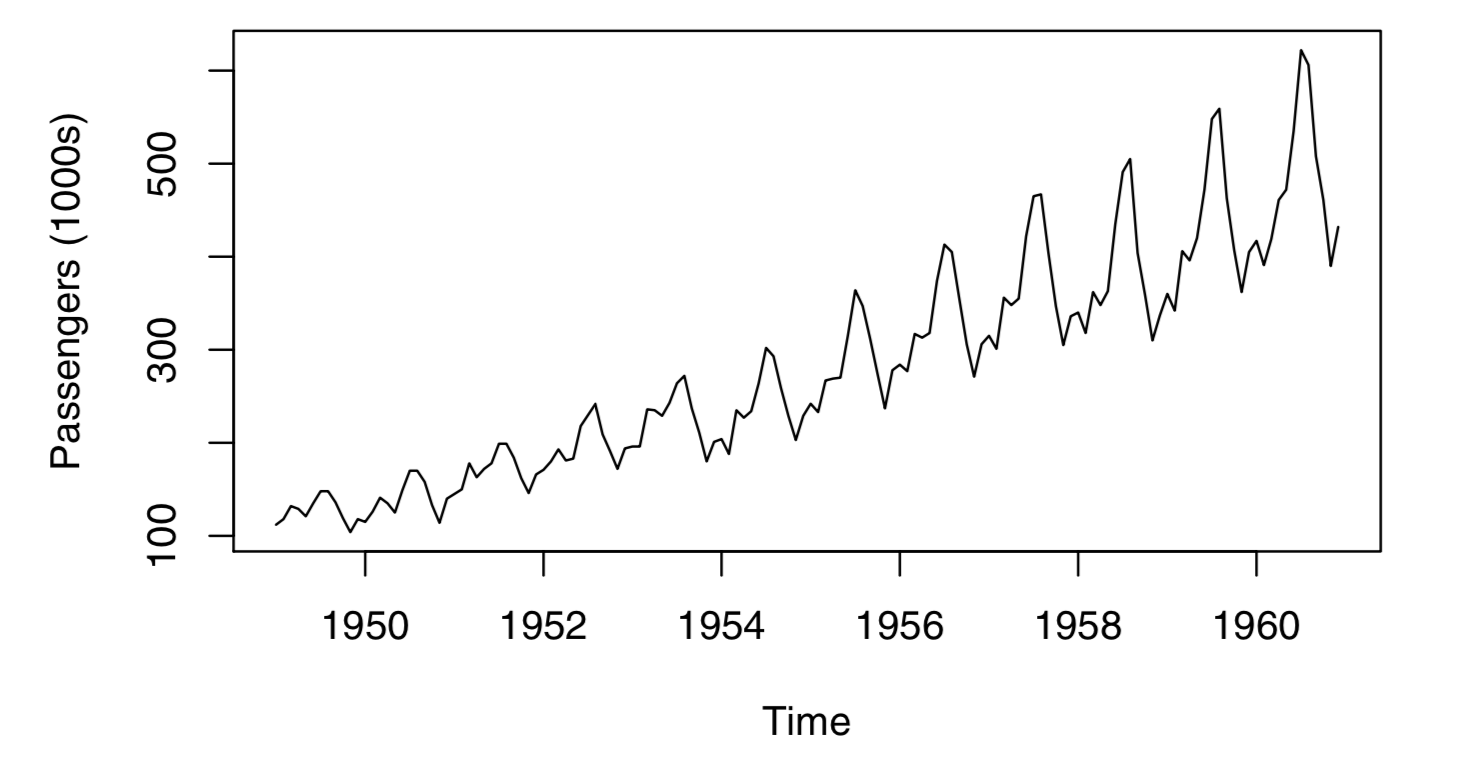
\includegraphics[scale=0.35]{src/TS-TREND.png}
		\item	The trend has many possible explanations (post-WWII prosperity, cheaper flights, etc.) but if there are non then it would be a \textbf{stochastic trend};
		\item[]	In this case, regression's not appropriate;
		\item	Forecasting uses extrapolation supposing trends continue at a slow pace;
		\item	Therefore, linear extrapolation is a reasonable approximation for a \textbf{few steps} ahead;
		\item[]	There's no empirical way to verify this, so we must explain the trend to justify extrapolation;
		\item	Forecasts beyond a year are thus better described as \textit{\textbf{scenarios}};
		\item	\textbf{Seasonal effects} can be \textit{removed} by \textit{aggregating to an annual basis} and evaluating the resulting time series;
		\item	Example of Chocolate/Beer/Electricity in Australia for \textit{Multiple Time Series};
		\item	Because autocorrelated series will often have the same trends and seasonal variations, they're often removed before comparison;
		\item	These trends will often be \textit{deterministic}
		\item[]	Australian population increase leads to an increase in electricity usage;
		\item	In contrast, finance will often have \textit{stochastic} trends;
		\item	Sometimes these can be modeled with a \textbf{random walk};
		\item	Idea of there being two distinct trends
		
		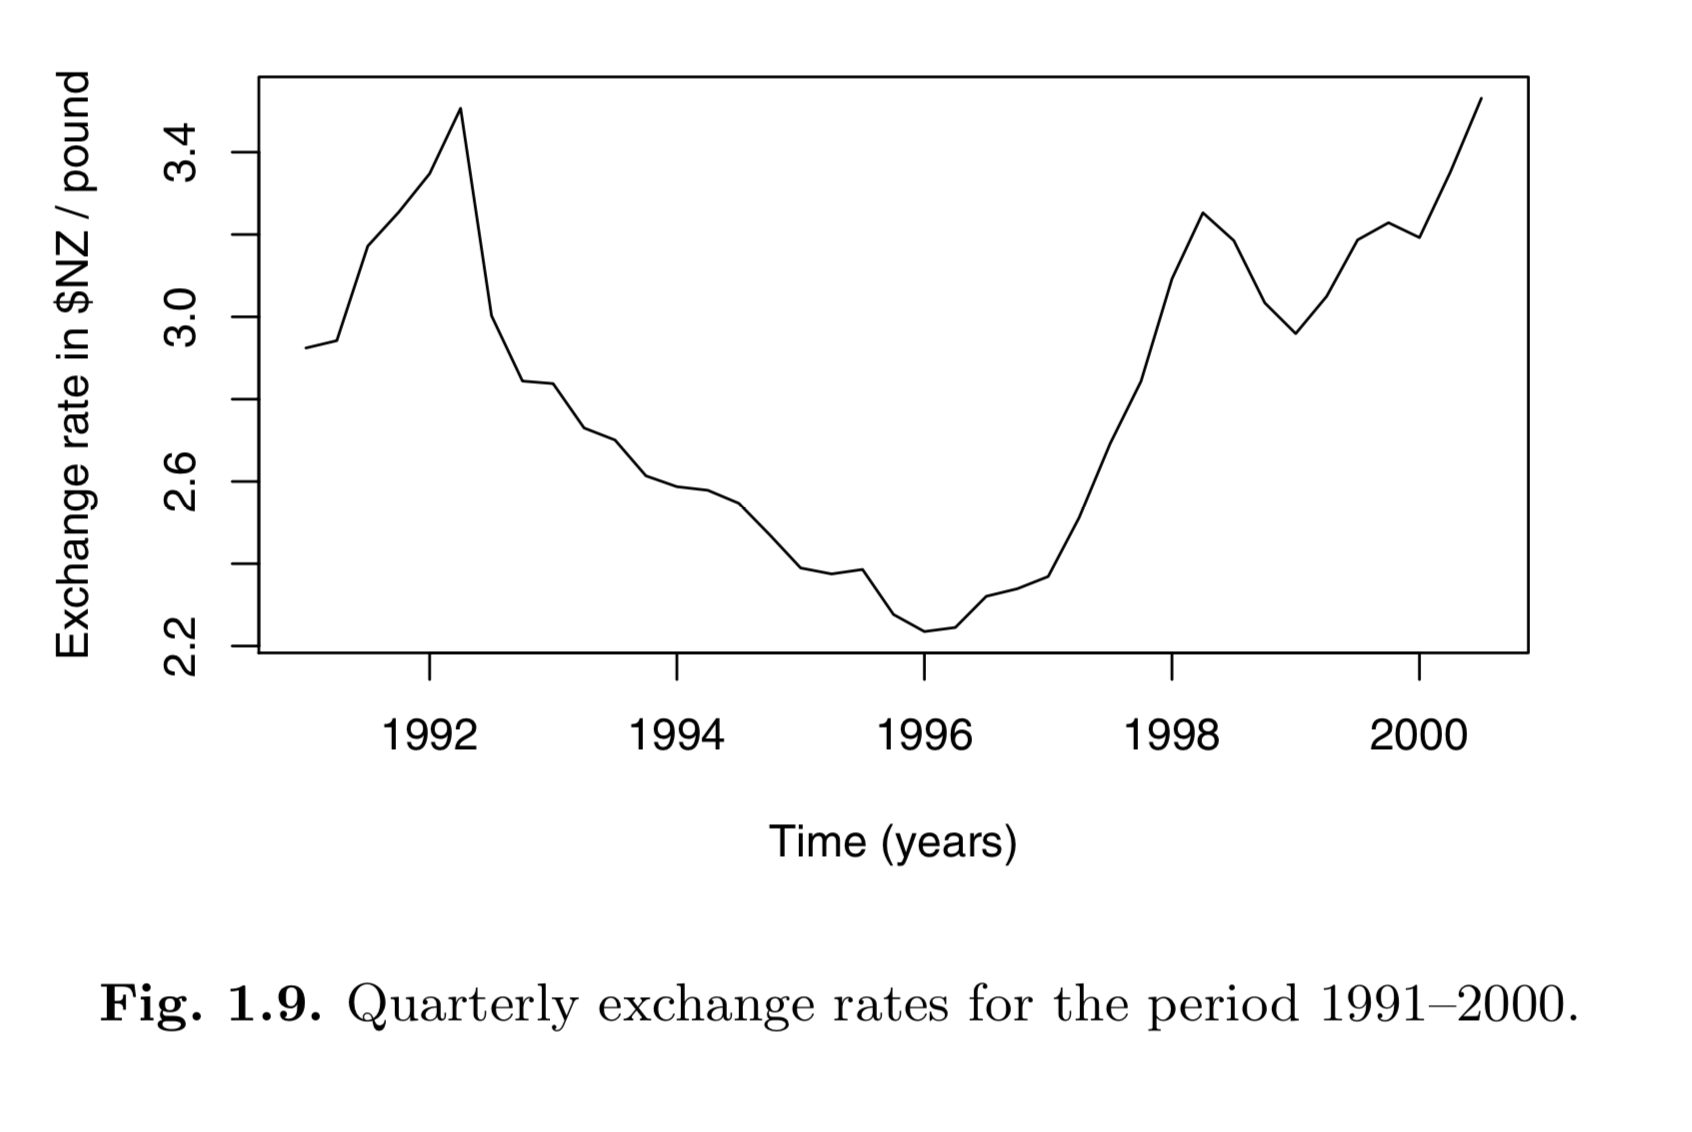
\includegraphics[scale=0.35]{src/TS-TREND-SPLIT.png}
		\item	Thereby, split the series in 2 (\texttt{window} in \texttt{R});
		
		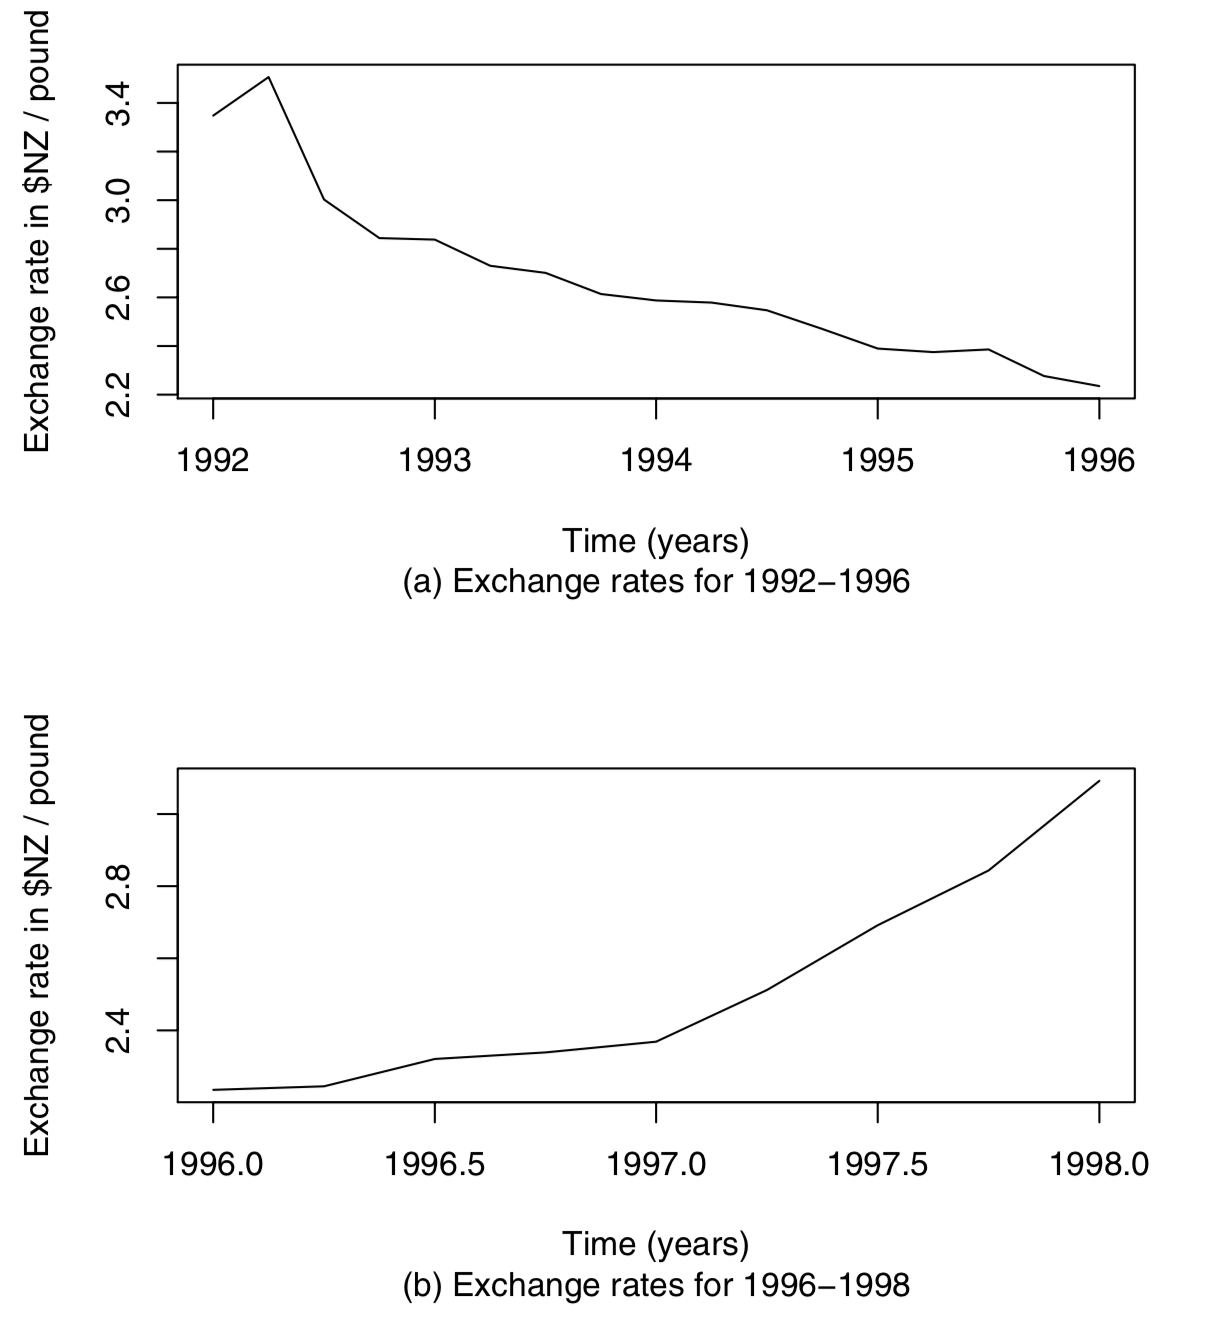
\includegraphics[scale=0.35]{src/TS-TREND-SPLIT-PLOTS.png}
		\item	This also highlights the importance of not extrapolating---without additional information we don't know whether the trend will continue;
		\item	Idea that 2 unrelated time series will be correlated if they both contain a trend thus we can't attribute global warming to fossil fuel increase without a physical explanation;
		\item	As per scientists, we judge appropriate to attribute a \textbf{causal relationship} and to expect mean global temperature to continue rising if greenhouse gas emissions aren't reduced;
		\end{itemize}
	\item[1.5:]	Time Series Data---Decomposition of series;
		\begin{itemize}
	\item	Time series of length $n$: $\{x_{t} : t = 1, \dots, n\} = \{x_{1}, x_{2}, \dots, x_{n}\}$;
	\item[]	It is a sequence of random variables $x_{t}$ sampled at $n$ discrete times $1, 2, \dots, n$;
	\item	Forecast at time $t$ for a future value $t + k$: $\hat{x}_{t + k | t}$;
	\item[]	$k$ is the \textbf{lead time};
		\end{itemize}
		\begin{itemize}
		\item	If the seasonal effect tends to increase as the trend increases, a multiplicative model may be more appropriate;
		\item	If there's a multiplicative factor modelled with the random variable (for example we have really large numbers) then an additive decomposition model for $\log(x_{t})$ may be more appropriate;
		\end{itemize}
		\begin{itemize}
		\item	Moving average centered around $x_{t}$ is one of the simplest ways to estimate a trend;
		\item[]	Because the average time is $t = 6.5$ and we have integer values, we have one half of both $x_{t - 6}$ and $x_{t + 6}$;
		\item	We can estimate the seasonal effect of each month $\bar{s}_{t}$ by averaging $\hat{s}_{t}$ per month;
		\item	Substracting these from the time series gives the \textbf{seasonally adjusted series};
		\end{itemize}
		\begin{itemize}
		\item	\textbf{loess}: locally weighted regression technique;
		\item[]	\og \textit{local} \fg{} as it uses a \og small \fg{}  number of points \og around \fg{}  it;
		\item[]	Thereby, this reduces the impact of outliers;
		
		\end{itemize}
\end{itemize}

\begin{FORMULA_SUMM}{Formules chapitre 1}
Notation:
	\begin{align*}
	\text{time series}&:	
		\{x_{t} : t = 1, \dots, n\} 
	= 	\{x_{1}, x_{2}, \dots, x_{n}\}	\\
	\text{forecast}	&:	
		\hat{x}_{t + k | t}
	\end{align*}
	
Models
	\begin{align*}
	\text{additive decomposition model}	:	
	x_{t}	
	&=	m_{t} + s_{t} + z_{t}		\\
	\text{multiplicative model}	:	
	x_{t}	
	&=	m_{t} \cdot s_{t} + z_{t}		\\
	\text{additive decomposition model for }\log(x_{t})	:	
	x_{t}	
	&=	m_{t} + s_{t} + z_{t}	\\
	\text{forecast when }z_{t} \sim \mathcal{N}(0, \sigma^{2})	:
	\hat{x}_{t}	
	&=	\text{e}^{m_{t} + s_{t}}\text{e}^{\frac{1}{2}\sigma^{2}}
	\end{align*}
où
	\begin{multicols*}{2}
	\begin{description}
	\item[$x_{t}$]	observed series;
	\item[$m_{t}$]	trend;
	\item[$s_{t}$]	seasonal effect;
	\item[$z_{t}$]	error term.
	\end{description}
	\end{multicols*}
$z_{t}$ is generally a sequence of random variables with a mean of zero;

Moving average of a monthly series
	\begin{align*}
	\hat{m}_{t}
	&=	\frac{\frac{1}{2} x_{t - 6} + x_{t - 5} + x_{t - 4} + x_{t - 3} + x_{t - 2} + x_{t - 1} + x_{t} + x_{t + 1} + x_{t + 2} + x_{t + 3} + x_{t + 4} + x_{t + 5} + x_{t + 6}}{12}	\\
	\end{align*}
	
Monthly additive effect estimation:
	\begin{align*}
	\hat{s}_{t} 
	&= 	x_{t} - \hat{m}_{t}	\\
	\end{align*}
	
Monthly multiplicative effect estimation:
	\begin{align*}
	\hat{s}_{t} 
	&= 	\frac{x_{t}}{\hat{m}_{t}}	\\
	\end{align*}
	
$\bar{s}_{t} = \text{mean}(\hat{s}_{t})$.


\end{FORMULA_SUMM}
\tcbline
	\begin{itemize}
		\item	
	\end{itemize}
\end{CHPT_SUMM_AUTO}

\begin{CHPT_SUMM_AUTO}[label = {L.-58}]{58. Time Series: Correlation}
Introduction to Time Series with \texttt{R} 2 - 3.1
\begin{itemize}
	\item[2:]	Correlation
	\item[3.1:]	Forecasting Strategies---Purpose
\end{itemize}
\tcbline
	\begin{enumerate}
		\item	Second order properties of a time series;
		\item	Relationships of different time series;
	\end{enumerate}
\end{CHPT_SUMM_AUTO}

\begin{CHPT_SUMM_AUTO}[label = {L.-59}]{59. Time Series: White Noise and Random Walks}
Introduction to Time Series with \texttt{R} 4.1 - 4.4
\begin{itemize}
	\item[4.1:]	Basic Stochastic Models---Purpose
	\item[4.2:]	Basic Stochastic Models---White Noise
	\item[4.3:]	Basic Stochastic Models---Random Walks
	\item[4.4:]	Basic Stochastic Models---Fitted models and diagnostic plots
\end{itemize}
\tcbline
	\begin{enumerate}
		\item	White noise;
		\item	Random walks;
	\end{enumerate}
\end{CHPT_SUMM_AUTO}

\begin{CHPT_SUMM_AUTO}[label = {L.-60}]{60. Time Series: Autoregressive Models}
Introduction to Time Series with \texttt{R} 4.5 - 4.8
\begin{itemize}
	\item[4.5:]	Basic Stochastic Models---AR models
	\item[4.6:]	Basic Stochastic Models---Fitted models
	\item[4.7:]	Basic Stochastic Models---Summary of \texttt{R} commands
	\item[4.8:]	Basic Stochastic Models---Exercices
\end{itemize}
\tcbline
	\begin{enumerate}
		\item[]	Correlograms and partial correlograms;
		\item[]	Stationnarity;
		\item[]	Forecasting with $AP(p)$ series;
	\end{enumerate}
\end{CHPT_SUMM_AUTO}

\begin{CHPT_SUMM_AUTO}[label = {L.-61}]{61. Time Series: Regression}
Introduction to Time Series with \texttt{R} 5
\begin{itemize}
	\item[5:]	Regression
\end{itemize}
\tcbline
	\begin{enumerate}
		\item	Correcting for autocorrelation;
		\item	Seasonality;
		\item	Logarithmic transformations;
		\item	Error correction factors;
	\end{enumerate}
\end{CHPT_SUMM_AUTO}

\begin{CHPT_SUMM_AUTO}[label = {L.-62}]{62. Time Series: Moving Average Models}
Introduction to Time Series with \texttt{R} 6.1 - 6.4
\begin{itemize}
	\item[6.1:]	Stationary Models---Purpose
	\item[6.2:]	Stationary Models---Strictly stationary series
	\item[6.3:]	Stationary Models---MA models
	\item[6.4:]	Stationary Models---Fitted MA models
\end{itemize}
\tcbline
	\begin{itemize}
		\item	
	\end{itemize}
\end{CHPT_SUMM_AUTO}

\begin{CHPT_SUMM_AUTO}[label = {L.-63}]{63. Time Series: ARMA Models}
Introduction to Time Series with \texttt{R} 6.5 - 6.8
\begin{itemize}
	\item[6.5:]	Stationary Models---Mixed models: The ARMA process
	\item[6.6:]	Stationary Models---ARMA models: Empirical Analysis
	\item[6.7:]	Stationary Models---Summary of \texttt{R} commands
	\item[6.8:]	Stationary Models---Exercices
\end{itemize}
\tcbline
	\begin{itemize}
		\item	
	\end{itemize}
\end{CHPT_SUMM_AUTO}

\begin{CHPT_SUMM_AUTO}[label = {L.-64}]{64. Time Series: ARIMA and SARIMA Models}
Introduction to Time Series with \texttt{R} 7.1 - 7.3
\begin{itemize}
	\item[7.1:]	Non-stationary Models---Purpose
	\item[7.2:]	Non-stationary Models---Non-Seasonal ARIMA models
	\item[7.3:]	Non-stationary Models---Seasonal ARIMA models
\end{itemize}
\tcbline
	\begin{itemize}
		\item	
	\end{itemize}
\end{CHPT_SUMM_AUTO}

\subsection{Notes sur les vidéos YouTube}

\begin{YTB_SUMM}[label = {SQ-BASICS-ML-INTRO}]{\href{https://www.youtube.com/watch?v=Gv9_4yMHFhI&list=PLblh5JKOoLUICTaGLRoHQDuF_7q2GfuJF&index=2&t=0s}{StatQuest: A Gentle Introduction to Machine Learning}}
\begin{itemize}
	\item	
\end{itemize}
\end{YTB_SUMM}

\newpage

\end{document}
